\chapter{Related Work}
\label{cha:relatedwork}

Revenue models on the Internet in order to monetize content is a topic that has been actively researched and experimented with over the past few decades. This chapter dives into the related work on both the technical and the economical level. It is structured in a way so that three different research areas will be discussed.
Firstly, the current widely adopted approaches, such as advertisements and subscriptions, are analyzed. Secondly, experimental systems that are using different ways to reward contentmakers, for example with automated payments, are investigated. Lastly, the new relevant possibilities that arise in the blockchain era are discussed.

\section{Technical solutions}

In order to generate revenue from online content, there are three technical solutions broadly adopted: online advertising, fee-based and donation-based systems.

\subsection{Online advertising}
Advertising is a method to draw attention to a product, service or event in order to promote sales or attendance \cite{stanton1994fundamentals}. Since the early days of the World Wide Web, this industry has also expanded to the Internet. The first advertisement on the Internet is possibly from 1994 on HotWired.com, which was bought by AT\&T and had a click through rate of 44\% \cite{firstbanner}. Meanwhile, the online advertising industry is very profitable and has almost evolved into the core business of the World Wide Web.

This section gives an overview of the current role model of the online advertisement industry and takes a closer look at the different approaches in the online advertising business and their privacy aspects. Lastly, the research field of privacy-friendly alternatives to advertisement networks are discussed.

Normally, there are multiple parties involved in the advertising ecosystem. On one side, there is a publisher, such as \textit{Der Spiegel} that provides online content, for example: news articles. On the other side, there is an advertiser that provides the advertisement.

\begin{figure}[h!]
  \center
  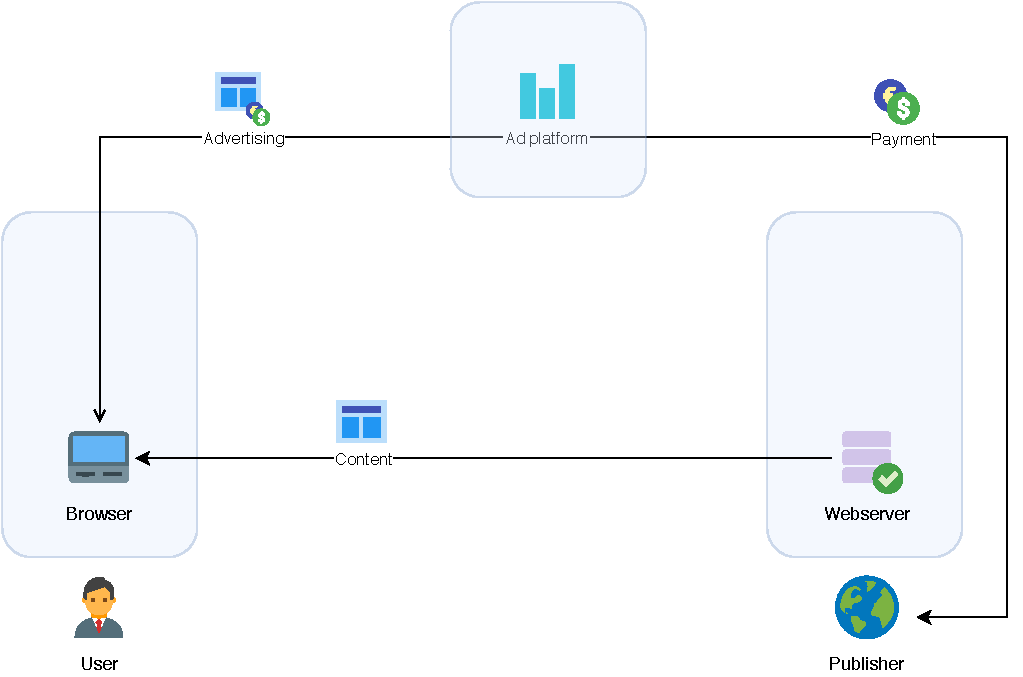
\includegraphics[width=12cm]{images/adplatform.pdf}
  \caption{Schematic overview of traditional ad platform}
\end{figure}

The most interesting part, however, is the ad platform. Ad platforms are entities that connect the publisher to the advertiser by providing them an interface to match both demand and supply. Due to the wide range of different publishers and users that are reached by ad networks, it becomes very efficient to allocate ad space. Ad platforms are even considered as the central hub in the online advertising industry \cite{estrada2017online}.

To make it possible for the ad platform to serve the right advertisements to the right user, the following methodology is applied: when a user visits the website of a publisher, the browser communicates with the webserver. The browser receives the content and displays it to the user. Along with this content, additional scripts that are associated with an ad network are also delivered to the browser and executed. These scripts are triggering a connection to the ad platform. The ad platform is able to serve extra commercial content (advertisements) over this connection, which is embedded into the page by the script. This method makes it possible for ad platforms to partner up with huge amounts of publishers and serve an amount of users that is several orders of magnitudes higher \cite{estrada2017online}.

The ad platform itself consist of multiple components, that might also be run by different entities. Firstly, there is an ad network, which resells the ad space from a publisher to an advertiser. Secondly, another component on the ad platform is the ad exchange. These are auction based advertisement marketplaces where advertisers can bid on ad space in real time. This means that the auction takes place when the user visits the website of the publisher. Based on the profile of the user, certain advertisers might be more interested to buy the ad space and thus offering a higher price \cite{estrada2017online}. Thirdly, a data aggregator is an entity which goal is to gather and aggregate data about the purchasing preferences of the users. This data is used to provide insights to both the advertisers and the publishers to target their marketing decisions \cite{estrada2017online}.

\subsubsection{Privad}
\label{sec:privad}
The problem with the infrastructure mentioned above, is that everything can be controlled by one single entity. Something that regularly happens as big players like Google are offering a one stop shop solution for both publishers and advertisers. This single entity knows everything about all parties involved: advertisers, publishers and users. The behavior of a single user is tracked across multiple websites, which might be considered a privacy concern. Guha et al. \cite{guha2011privad} developed Privad, which they call a practical private online advertising system.

The model of Privad is slightly different from the original online advertising role model. This model includes likewise the user, publisher and advertiser. However, in this model there are also a dealer and a broker present. One key difference compared to the traditional online advertising model is that the profiling (building a profile of the user based on interests) is done on the users' computer and not by a central data aggregator. Secondly, the ad platform is split into two different entities: the broker and the dealer. The broker is comparable to the traditional ad platform and matches the user profile with advertisements. The request, however does not come from the users' computer immediately: there is a dealer placed in between. The dealer anonymizes every request before it is sent to the broker and makes sure that click fraud is prevented. The dealer cannot eavesdrop on the request, because the request is sent in an encrypted form to the broker \cite{guha2011privad, bilenko2011targeted}.

\begin{figure}[htbp]
  \centering
      \includegraphics[clip, page=3, trim=0.5cm 18.5cm 11.9cm 1cm, width=9cm]{assets/privad-performance.pdf}
  \caption{Privad overview \cite{guha2011privad}}
  \label{fig:somthing}
\end{figure}

One concern with this approach is that a profile might be so detailed that the broker is able to find out an identity based on the profile. In order to tackle this problem, Privad works with a subscription to a certain general profile that is shared with multiple other users. The user receives multiple advertisements and can pick locally which suits best.

Trust, however is still a key element in this approach. There is no way to find out if the dealer is trustworthy. If the dealer and the broker are secretly run by the same entity, it is possible to exchange data and learn more about the user.

\subsection{Fee-based}

The second business model that is being used as an alternative to online advertising is requiring payments in exchange for content. This section describes what different approaches there are in the field of online payments and subscription models.

\subsubsection{Subscriptions}

Even in the early days of the World Wide Web, the phenomenon of content that can only be consumed with a subscription existed. Such a mechanism is called a paywall. For example, the \textit{Wall Street Journal} implemented already a hard paywall in 1996, which is still in place today and has over 2 million subscribers as of February 2020 \cite{firstpaywall}.
Alternatives to hard paywalls are soft paywalls. The difference between both types is that soft paywalls are trying to convince potential customers to subscribe by giving them a free sample of the content. For example, the \textit{New York Times} has implemented a soft paywall with a limit of five free articles per month \cite{cook2012paying}.

% Salwen, Michael B.; Garrison, Bruce; Driscoll, Paul D. (2004). Online News and the Public. Routledge. p. 136. ISBN 978-1-135-61679-3.

Paywalls however, are fairly easy to circumvent. This is especially the case for soft paywalls. Therefore, publishers are trying to implement counter measures in order to enforce a subscription. For example, the \textit{New York Times} attacked one popular circumvention method: the use of an incognito window in order to prevent the free articles from being counted. With behavioral analysis, it is possible to find out that the user is using an incognito window, which enables the \textit{New York Times} to prevent the free article from being served \cite{troupson2015yes}.

\subsubsection{Micropayments}
Micropayments are already widely adopted by a younger target audience as it used in order to pay for mobile content like apps and music. In the last decade, micropayments are also applied as an alternative to the subscription model offered by online publishers. Since the value of a micropayment is generally just a couple of cents, credit or debit card payments are not suitable due to high transaction costs. Several companies have entered the field of micropayments in order to offer cheap and easy to use micropayment solutions. The application of micropayments in the publishing industry, however, affects the way users are interacting with the medium \cite{geidner2015effects}.

First of all, there is a difference between monetary and non-monetary micropayments. Monetary means that the payment is made via the transfer of a currency. For example, Google Checkout and Paypal are offering such a service. With the non-monetary variant, the user pays with a small amount of knowledge or labor. An example of such a non-monetary micropayment system is the Google Surveys product. When a user visits an article that requires a non-monetary payment, a survey question needs to be answered first before the access to the article is granted. The publisher gets paid around 0.05 USD per answered survey question. The surveys are used by market analysts who are paying Google in order to get the survey responses \cite{googlesurveys}.

Even before the widespread introduction of micropayment solutions, researchers warned that buying something does not only cost money but also requires extra effort compared to free content, because the user needs to estimate the value in advance. This phenomenon is called mental transaction costs \cite{szabo, shirky, oh2016free}. Secondly, a problem with the competition from free content is that it is a ``stable strategy'', which means that there is no competition other than paying your visitors for reading your website, which is very unlikely to succeed in the long term. Thirdly, a problem with online content is that it is hard to value because information is hard to value in advance. The combination of mental transaction costs, the competition from free sources and a product that is hard to value, makes micropayments very unlikely to be profitable for online content \cite{shirky}.

\subsection{Donation-based}

Other publishers are relying on the willingness of their users to compensate. These systems are either implemented on one particular website or offered as a service over multiple websites.

The Wikimedia Foundation is an example of a non-profit organization that actively asks for donations on their Wikipedia website; nonetheless, this is not the main source of their revenue, because big companies like Amazon or Google are donating large sums to the foundation. Wikimedia raised a total of 91M USD in 2016-2017 \cite{wikimediadonation}.

For smaller websites, such a campaign is not very viable. Users are not likely to send a donation to each individual contentmaker they support. For these minor publishers, Flatter\footnote{\url{https://flatter.com}} offers a user experience which is similar to the Facebook-like button. Although, the difference is that instead of just showing the interest in a certain page of website, the button also shows appreciation by making a small micropayment. Flatter offers a subscription with a minimum of 2 EUR per month. This monthly subscription fee is divided amongst all websites the user clicked the Flatter-button on \cite{loll2010flattr}. Using such a centralized service comes with privacy concerns, as Flattr is able to track the browsing behavior of connected users and publishers.

\section{Automated payments}
As advertisements are suboptimal from a privacy, security and user experience perspective, companies are looking for alternatives. In 2016, Brave Software launched a browser that blocks ads and trackers by default: the Brave Browser\footnote{\url{https://www.brave.com}}. During the introduction, Brave Software also shared their plans for a Brave Publisher Ads program which pays publishers a fair share of their Internet revenue. As of 2020, their service is called ``Brave Rewards Program'', in which any content creator can enroll in order to get paid for content. The following section discusses the technical aspects and privacy measures of this system.

\subsection{Brave Rewards}
\label{sec:brave}
In order to build a system that makes it possible to reward content makers on the Internet, Brave Software introduced the Basic Attention Token (BAT) \cite{token2018blockchain,locklin2018token}. This token, which works like any other cryptocurrency, represents user attention. Their goal with this token is to trade ``attention'' just like any other commodity, like oil and coffee. This means that this token can also be traded on a cryptocurrency exchange. Brave Software is promoting this token to use it to reward Internet users. What happens is that the Brave Browser is equipped with a standard ad blocker. The websites are filled with sponsored content by the Brave Browser. The difference with the original advertisements is that the user gets rewarded for viewing them by receiving BAT-tokens. The BAT-token can be traded for other crytocurrencies or even fiat currencies.

For this research, another application of the BAT-token is even more interesting. That is, the system also works the other way around: users can spend their BAT-tokens on websites of the publishers they support in an automated manner. The remainder of this section shows the inner working of this system. Furthermore, it explains why even that is still suboptimal from a decentralized perspective. First, the concept of the Brave Vault is explained. Secondly, the privacy and anonymity measures are analyzed. Lastly, the monopoly of Brave Software in this ecosystem is discussed.

The Brave Vault is a private datastore where browsing information is stored. The central part in this Brave Vault is the \textit{persona}, that is used to identify and set your browsing behavior. The \textit{persona} can be synced with other browsers, so that one user still uses the same profile when switching devices. Another part of the Brave Vault is the \textit{session}. The \textit{session} is bound to the browser and does not have a predefined lifetime. Browser dependant information, like browsing history, is stored here \cite{brave-vault}.

In the \textit{persona}, there is a setting that enables an ad-free browsing experience by paying a small contribution. The contribution amount is divided amongst the websites that the users visits. However, if these contributions are sent to the publishers directly, it would be very hard to guarantee privacy and anonymity. Based on the contributions, it is possible to reconstruct a profile that might be linked to an individual. To tackle these privacy concerns, Brave Software developed the Brave Ledger \cite{bat-ledger}. The Brave Ledger is a central system that processes micropayments for the contributions to the publishers. The system is designed on two core principles: anonymity and accountability. The former means that Brave Software should not be able to correlate publisher visits with contributions. The latter implies that Brave Software should only be able to have insights in the contributions on an aggregated basis.

In order to build a system on these principles, the Brave Ledger combines statistical voting with an anonymous voting scheme \cite{bat-ledger}. First, statistical voting means that if you only have one vote, but you would like to vote on multiple choices, you are picking a choice at random out of your preferred choices. If everyone follows this system, the result of the election would be roughly the same as if everyone had multiple votes. The benefit of combining such a system with making contributions to certain publishers, is that the user is not revealing his entire browsing history, but only one publisher he wants to reward. One vote reflects a payment towards one publisher. Secondly, the Brave Ledger makes use of an anonymous voting scheme called ANONIZE2 \cite{hohenberger2014anonize, hohenberger2015overview}. This system guarantees that every single user in a group of users is able to cast a maximum of one vote, while keeping the vote anonymous.

Brave Software used an initial coin offering to introduce the new token to the market. The ICO happened in May 2017 and raised 156,000 ETH, which was worth around 35M USD at the time. The raised money is mostly used to pay for the development and other costs of the token. The development team exists out of 20 developers. However, the main problem with the BAT-ecosystem, is that there are a couple of points where Brave Software acts as a central authority. It is only possible to enroll in the program for ``verified publishers'', which is up to Brave Software to decide. This makes the system not decentralized at all.

\section{Blockchain}

Blockchain technology has been with us for more than a decade. Satoshi Nakamoto built the first practical application that used the so-called blockchain as a decentralized ledger, where it is possible to transfer a digital currency without trusting a single party \cite{nakamoto2019bitcoin}. Since then, a lot has changed and all kinds of experiments using this technology are performed. For example, blockchain implementations are now capable of running scripts which are even Turing complete, which opens the door to programmable money \cite{wood2014ethereum} and all kinds of other assets that can be stored on the blockchain.

\subsection{Lightning Network}
\label{sec:lightning}
The general problem with blockchain technology is scalability and speed: the current average confirmation time of a Bitcoin transaction takes a couple of minutes \cite{bamert2013have}. With the current blocksize of 1MB, the amount of transactions is limited to seven per second. Therefore this technology is not suitable for micropayments, which are payments with a value less than a dollar \cite{definitionmicropayment}.

In order to solve this problem, several researchers have experimented with alternative ways to circumvent these issues. The most promising system in this research field is the Lightning Network \cite{poon2016bitcoin}. The goal of the Lightning Network is to send small payments immediately, without intervention of the blockchain ledger and with minimal fees. The Lightning Network features such a system by combining a smart idea with the capabilities of multi signature addresses. 

To understand the system, the following example is given: The system relies on two parties, for example Alice and Bob, opening a joint account (channel). Off-chain, there is an agreement on which part of the joint account belongs to whom. With this joint account, Alice can transfer money to Bob and vice versa by just updating this agreement about the joint account. However, it is still not very practical if Alice also needs to open a joint account with any other party, for example Charlie, that she wants to transfer money to. The Lightning Network solves this issue by finding a path from Alice to Charlie using multiple joint accounts. In this example, it might be the case that Charlie has a joint account with Bob. Using these two joint accounts, Alice can transfer money indirectly to Charlie via Bob. In practice, this system follows a hubs and spokes model, where a couple of big players are connected to a lot of individuals in order to create a reliable network. Every hop that is used by a single transaction can also receive a small fee, but these fees are insignificant compared to on-chain transactions \cite{poon2016bitcoin}.

